\documentclass{article}
\usepackage[utf8]{inputenc}
\usepackage{hyperref}
\usepackage{amsmath}
\usepackage{amsfonts}
\usepackage{graphicx}
\usepackage{enumitem}
\usepackage{wrapfig}
\graphicspath{ {./images} }


\title{Diagnostic}
\author{
    Tan Chien Hao\\
    \texttt{www.tchlabs.net}\\
    \texttt{Telegram @tch1001}
    % new collaborators add your name and contact here!
}

\date{\today}
\begin{document}
\newif\ifpaper

% TOGGLE ANSWER HERE
\paperfalse 

\maketitle

\begin{samepage}
\subsubsection{Kinematics: SJPO 2016 General Round Q8}
A train moving on straight horizontal tracks slows down from $66 \mathrm{~ms}^{-1}$ to $22 \mathrm{~ms}^{-1}$ at a constant rate of $2.0 \mathrm{~ms}^{-2}$. What distance does it travel while slowing down?
\begin{itemize}
\item[](A) $490 \mathrm{~m}$
\item[](B) $650 \mathrm{~m}$
\item[](C) $740 \mathrm{~m}$
\item[](D) $970 \mathrm{~m}$ 
\item[](E) $1100 \mathrm{~m}$ \end{itemize}
Ans: \ifpaper D \fi
\end{samepage}

\begin{samepage}
\subsubsection{Vectors: SJPO 2015 General Round Q11}
A force $\vec{F} = \vec{F}_1 + \vec{F}_2$ can be decomposed as the sum of 2 vectors $\vec{F}_1$ and $\vec{F}_2$. Only the magnitude of $\vec{F}_1$ and the direction of $\vec{F}_2$ are known. Which of the following is the most accurate statement?
\begin{itemize}
\item[](A) Only one combination of $\vec{F}_1$ and $\vec{F}_2$ exists.
\item[](B) There exists exactly two combinations of $\vec{F}_1$ and $\vec{F}_2$.
\item[](C) There exists infinite combinations of $\vec{F}_1$ and $\vec{F}_2$.
\item[](D) At least three combinations of $\vec{F}_1$ and $\vec{F}_2$ exist but the total number of combinations is finite.
\item[](E) Only one or two combinations of $\vec{F}_1$ and $\vec{F}_2$ exist.
\end{itemize}
Ans: \ifpaper E \fi
\end{samepage}

\begin{samepage}
\subsubsection{Projectile Motion: SJPO 2016 General Round Q11}
A projectile is launched at velocity $v_0$ into an ideal ball istic trajectory from the origin of a coordinate system. Given that: when the launch angle is varied, all the possible points that can be hit by the projectile are exactly contained within a parabola with equation $y=a+b x^2$ where $y$ is the vertical height, $x$ is the horizontal displacement from the origin, while $a$ and $b$ are constants. What could be the expression for $a$ and $b$ ?\\
 \begin{wrapfigure}{r}{0.4\textwidth} 
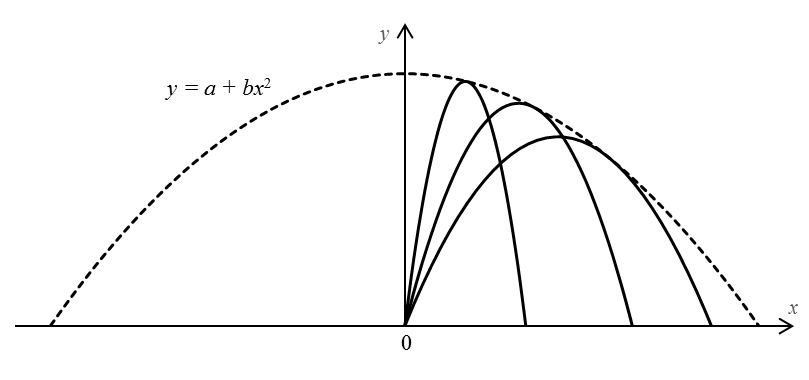
\includegraphics[width=\linewidth]{images/sjpo2016q11.png}
\end{wrapfigure}
\begin{itemize}
\item[](A) $\quad a=\frac{v_0{ }^2}{2 g}, b=\frac{g}{v_0{ }^2}$
\item[](B) $\quad a=\frac{v_0{ }^2}{2 g}, b=\frac{g}{2 v_0{ }^2}$
\item[](C) $\quad a=\frac{v_0{ }^2}{2 g}, b=\frac{2 g}{v_0{ }^2}$
\item[](D) $\quad a=\frac{v_0{ }^2}{g}, b=-\frac{g}{v_0{ }^2}$
\item[](E) $\quad a=\frac{v_0{ }^2}{2 g}, b=-\frac{g}{2 v_0{ }^2}$
\end{itemize}
Ans: \ifpaper E \fi \\[10pt]
Extra: Prove that the envelope is a parabola. \url{https://en.wikipedia.org/wiki/Envelope_(mathematics)}
\end{samepage}

\begin{samepage}
\subsubsection{Simple Harmonic Motion: SJPO 2015 General Round Q16}
As shown in the diagram, a pendulum of length $L$ is hung from the ceiling and at a point $P$, a peg is placed. $L^{\prime}$ denotes the shortened length of the pendulum during part of its oscillation. The period of the pendulums oscillation is now
\begin{wrapfigure}{r}{0.4\textwidth}
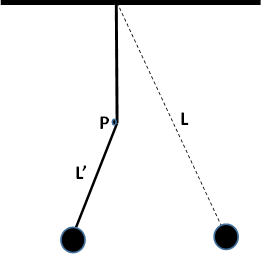
\includegraphics[width=0.9\linewidth]{images/2015q16.png}
\end{wrapfigure}
\begin{itemize}
\item[](A) $2 \pi \sqrt{\frac{L}{g}}$
\item[](B) $2 \pi \sqrt{\frac{L^{\prime}}{g}}$
\item[](C) $2 \pi\left[\sqrt{\frac{L}{g}}+\sqrt{\frac{L^{\prime}}{g}}\right]$
\item[](D) $\pi\left[\sqrt{\frac{L}{g}}+\sqrt{\frac{L^{\prime}}{g}}\right]$
\item[](E) $\pi \sqrt{\frac{L+L^{\prime}}{g}}$
\end{itemize}
Ans: \ifpaper D \fi
\end{samepage}


\end{document}